\documentclass[unicode,11pt,a4paper,oneside,numbers=endperiod,openany]{scrartcl}
\usepackage{amsmath}
\usepackage{amssymb}
\usepackage{ifthen}
\usepackage[utf8]{inputenc}
\usepackage{graphics}
\usepackage{graphicx}
\usepackage{hyperref}

\pagestyle{plain}
\voffset -5mm
\oddsidemargin  0mm
\evensidemargin -11mm
\marginparwidth 2cm
\marginparsep 0pt
\topmargin 0mm
\headheight 0pt
\headsep 0pt
\topskip 0pt        
\textheight 255mm
\textwidth 165mm

\newcommand{\duedate} {}
\newcommand{\setduedate}[1]{%
\renewcommand\duedate {Due date:~ #1}}
\newcommand\isassignment {false}
\newcommand{\setassignment}{\renewcommand\isassignment {true}}
\newcommand{\ifassignment}[1]{\ifthenelse{\boolean{\isassignment}}{#1}{}}
\newcommand{\ifnotassignment}[1]{\ifthenelse{\boolean{\isassignment}}{}{#1}}

\newcommand{\assignmentpolicy}{
\begin{table}[h]
\begin{center}
\scalebox{0.8} {%
\begin{tabular}{|p{0.02cm}p{16cm}|}
\hline
&\\
\multicolumn{2}{|c|}{\Large\textbf{HPC Lab for CSE 2024 ---  Submission Instructions}}\\
\multicolumn{2}{|c|}{\large\textbf{(Please, notice that following instructions are mandatory: }}\\
\multicolumn{2}{|c|}{\large\textbf{submissions that don't comply with, won't be considered)}}\\
&\\
\textbullet & Assignments must be submitted to \href{https://moodle-app2.let.ethz.ch/course/view.php?id=22516}{Moodle} (i.e. in electronic format).\\
\textbullet & Provide both executable package and sources (e.g. C/C++ files, Matlab). 
If you are using libraries, please add them in the file. Sources must be organized in directories called:\\
\multicolumn{2}{|c|}{\textit{Project\_number\_lastname\_firstname}}\\
& and  the  file must be called:\\
\multicolumn{2}{|c|}{\textit{project\_number\_lastname\_firstname.zip}}\\
\multicolumn{2}{|c|}{\textit{project\_number\_lastname\_firstname.pdf}}\\
\textbullet &  The TAs will grade your project by reviewing your project write-up, and looking at the implementation 
                 you attempted, and benchmarking your code's performance.\\

\textbullet & You are allowed to discuss all questions with anyone you like; however: (i) your submission must list anyone you discussed problems with and (ii) you must write up your submission independently.\\
\hline
\end{tabular}
}
\end{center}
\end{table}
}
\newcommand{\punkte}[1]{\hspace{1ex}\emph{\mdseries\hfill(#1~\ifcase#1{Points}\or{Points}\else{Points}\fi)}}


\newcommand\serieheader[6]{
\thispagestyle{empty}%
\begin{flushleft}

\includegraphics[width=0.4\textwidth]{ETHlogo_13}
\end{flushleft}
  \noindent%
  {\large\ignorespaces{\textbf{#1}}\hspace{\fill}\ignorespaces{ \textbf{#2}}}\\ \\%
  {\large\ignorespaces #3 \hspace{\fill}\ignorespaces #4}\\
  \noindent%
  \bigskip
  \hrule\par\bigskip\noindent%
  \bigskip {\ignorespaces {\Large{\textbf{#5}}}
  \hspace{\fill}\ignorespaces \large \ifthenelse{\boolean{\isassignment}}{\duedate}{#6}}
  \hrule\par\bigskip\noindent%  \linebreak
 }

\makeatletter
\def\enumerateMod{\ifnum \@enumdepth >3 \@toodeep\else
      \advance\@enumdepth \@ne
      \edef\@enumctr{enum\romannumeral\the\@enumdepth}\list
      {\csname label\@enumctr\endcsname}{\usecounter
        {\@enumctr}%%%? the following differs from "enumerate"
	\topsep0pt%
	\partopsep0pt%
	\itemsep0pt%
	\def\makelabel##1{\hss\llap{##1}}}\fi}
\let\endenumerateMod =\endlist
\makeatother




\usepackage{textcomp}






\begin{document}


\setassignment
\setduedate{Wednesday 26 June 2024, 23:59}

\serieheader{AI in the Sciences and Engineering}{Spring Semester 2024}
            {Student: Carla Judith L\'opez Zurita}
            {}{Project 3}{}
\newline

The main objective of the project is to apply the concepts learned in class
related to Neural Differential Equations and Hybrid Workflows.


\section{Inverted pendulum}\label{sec:task1}
The objective of this task is to control the inverted pendulum problem using a
Neural Network. The inverted pendulum is a classic problem in control theory,
where the goal is to balance a pendulum in an upright position by applying an 
external force $F$ to the cart that holds the pendulum. 
The system is described by the following differential equation:
\begin{align}
    (M+m) \ddot{x} + m l \ddot{\theta} \cos(\theta) - m l \dot{\theta}^2 \sin(\theta) = F \\
    l \ddot{\theta} + g \sin(\theta) + \ddot{x} \cos(\theta) = 0
\end{align}
where $\theta$ is the angle of the pendulum with respect to the vertical,
$g=9.81$ m/s$^2$ is the acceleration due to gravity, $l=1.0$ m is the length of
the pendulum, $m=0.1$ kg is the mass of the pendulum, $M=1.0$ kg is the mass of
the cart and $F$ is the force applied to the cart in Newtons.

\subsection*{Solving the coupled ODE system}
First, we need to solve the coupled ODE system to simulate the dynamics of the
inverted pendulum.
The idea is to use an autodifferentiation library to code the solver in order to
use it later to train a Neural Network to control the pendulum. In this case, I
used torch due to its familiarity to me.
I used Runge-Kutta 4th order method to solve the system. To test the
implementations, I simulated the system with a sinusoidal force $F(t) = 10
\sin(t)$.
The results are shown in Figure~\ref{fig:pendulum}.
\begin{figure}[h]
    \centering
    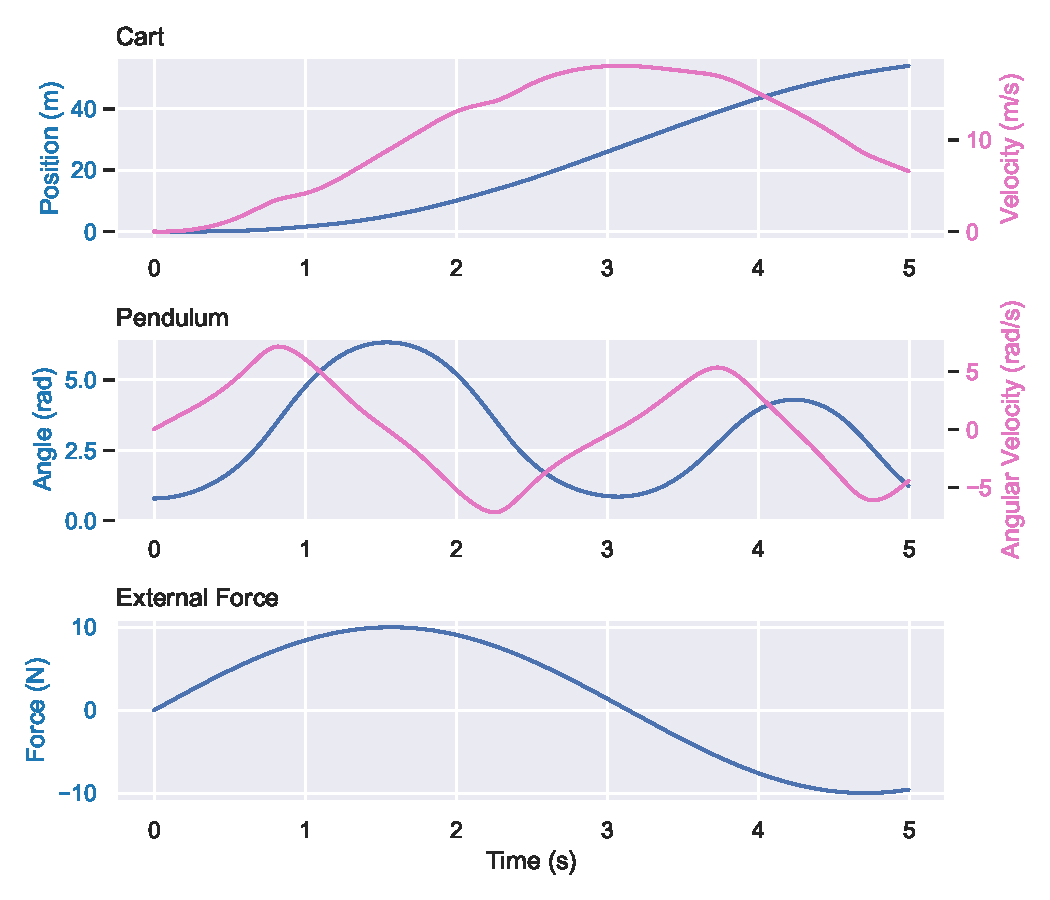
\includegraphics[width=0.8\textwidth]{../Task1/pendulum.pdf}
    \caption{Simulation of the inverted pendulum with a sinusoidal force.}
    \label{fig:pendulum}
\end{figure}

\subsection*{Learning to balance the pendulum}
Next, we will use a Neural Network to learn to balance the pendulum. The input
to the network will be just the time $t$ and the output will be the force $F$
applied to the cart. We will train the network using the whole trajectory of the
pendulum. The network will be trained using the Adam optimizer and a custom loss
function that penalizes the deviation of the pendulum from the vertical position
and large angular velocities. The network is a simple feedforward network with
1 hidden layer with 32 neurons and SiLU activation function. The output layer
has a single neuron with linear activation function. The network is trained for
500 epochs with an initial learning rate of $10^{-2}$ and a scheduler that
reduces the learning rate by a factor of 0.5 every 75 epochs.
The plot of the loss function during training is shown in Figure~\ref{fig:loss}.
\begin{figure}[h]
    \centering
    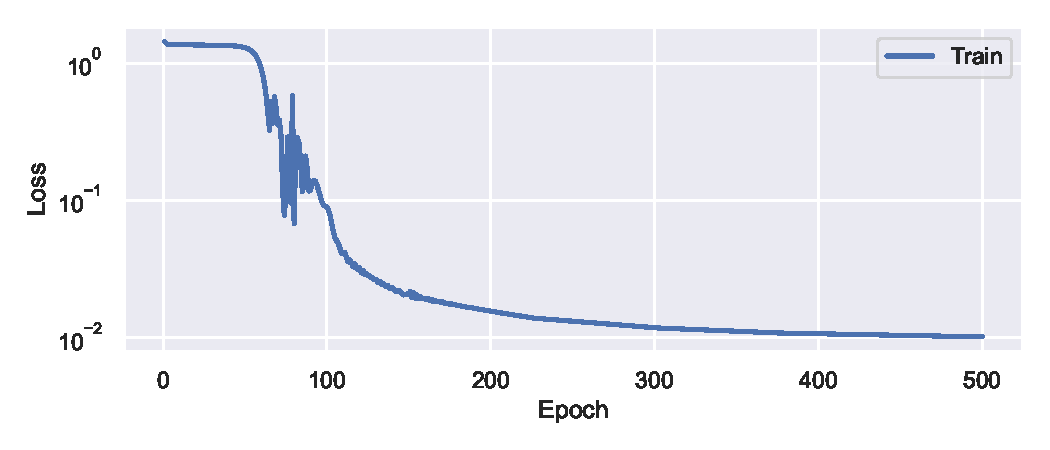
\includegraphics[width=0.8\textwidth]{../Task1/loss_function.pdf}
    \caption{Loss function during training of the Neural Network.}
    \label{fig:loss}
\end{figure}
The results of the simulation using the Neural Network to control the force
applied to the cart are shown in Figure~\ref{fig:pendulum_nn}.
\begin{figure}[h]
    \centering
    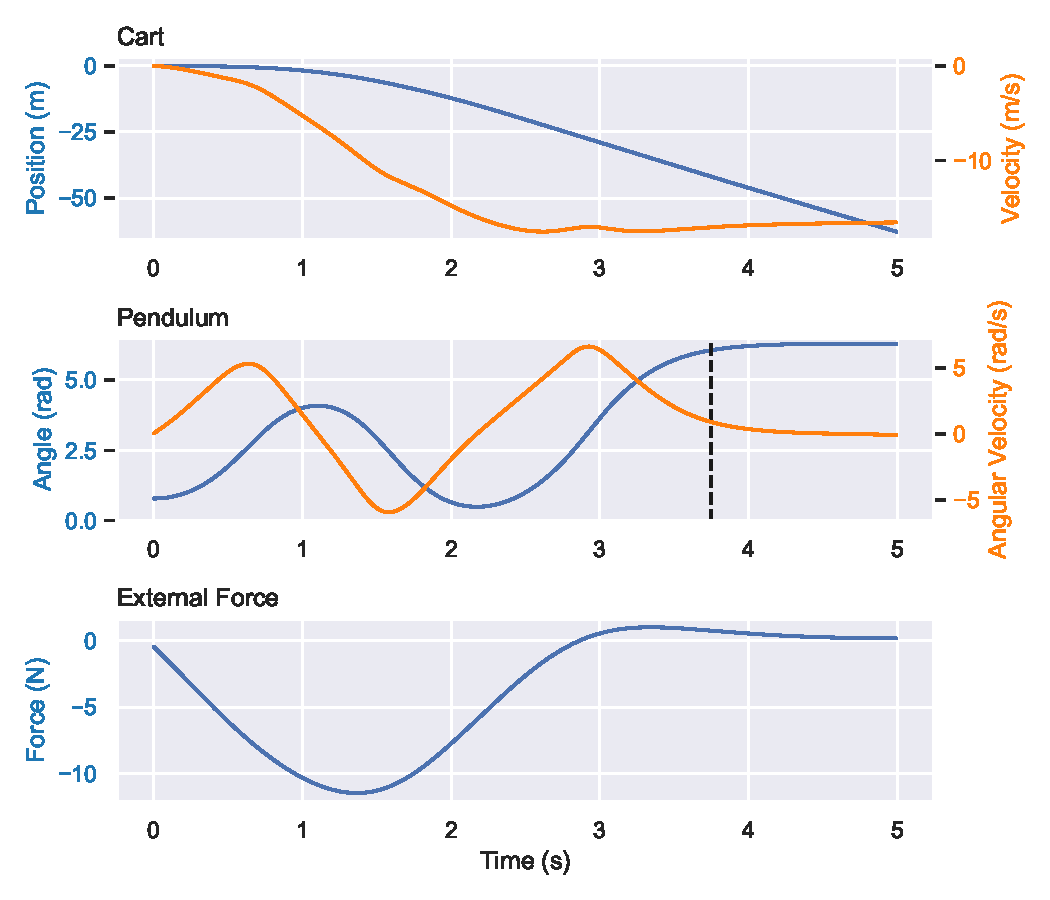
\includegraphics[width=0.8\textwidth]{../Task1/pendulum_nn.pdf}
    \caption{Simulation of the inverted pendulum using a Neural Network to
    control the force applied to the cart.}
    \label{fig:pendulum_nn}
\end{figure}

Attatched to the report you will find the code used to solve the ODE system and
train the Neural Network, as well as the simulation results in a gif format.

\section{PDE-FIND}\label{sec:task2}
The objective of this task is to use the PDE-FIND~\cite{PDEFIND} to discover the
differential equation that governs the dynamics of the some unkown system using
only data files.

The idea is that we can assume that the dynamics of the system can be described
by a partial differential equation of the form:
\begin{align}
    u_t = F(u, u_x, u_{xx}, u_y, u_{yy}, u_{xy}, \ldots, x, y, \ldots, t)
\end{align}
So we can create a library of possible functions that can appear in the right
hand side of the equation and use the data to find the coefficients of the
functions that best describe the dynamics of the system.

We are given three files with data of differents system for which we want to
find the PDE that governs the dynamics.

\subsection*{Implementation of PDE-FIND}
We will use the library PySINDy to use the PDE-FIND
algorithm. 

\subsection*{File 1}
The first file is a 1+1D dimensional system $u$, with $x$ and $t$ coordinates.

\subsection*{File 2}
The first file is also a 1+1D dimensional system $u$, with $x$ and $t$ coordinates.
\subsection*{File 3}
The third file is a 2+1D dimensional system, with $x$, $y$ and $t$ coordinates.


\section{Bonus Task}\label{sec:task3}


\bibliographystyle{plain}
\bibliography{bibliography}

\end{document}
